\documentclass[aspectratio=169]{beamer}

\usetheme{Madrid}
\usecolortheme{DSLAB}
\usefonttheme[onlylarge]{structurebold}
\setbeamerfont*{frametitle}{size=\normalsize,series=\bfseries}
\setbeamertemplate{navigation symbols}{}

\usepackage[utf8]{inputenc}
\usepackage[T1]{fontenc}
\usepackage{xmpmulti}
\usepackage{tikz}
\usepackage{pgf}
\usepackage{amsmath}
\usepackage{amsfonts}
\usepackage{graphicx}
\usepackage{color}
\usepackage{multirow}
\usepackage{lmodern}
\usepackage{hyperref}
\usepackage{eurosym}
\usepackage{listings}
\usepackage{array}

\lstset{
  basicstyle=\ttfamily\small,
  frame=single,
  breaklines=true,
  showstringspaces=false,
  columns=fullflexible
}


\usetikzlibrary{arrows}
\tikzstyle{block}=[draw opacity=0.7,line width=1.4cm]

\setbeamercovered{dynamic}
\setbeamerfont{author}{family=\rmfamily}
\institute[URJC]{DSLAB}

\author[Big Data Processing II]{
	Alberto Fernández Isabel \\
	Natalia Madrueño Sierro \\
	Rubén Rodríguez Fernández \\
}

\title[Presentación]{
	Big Data Processing II \\ \vspace{0.2em}
	IA Generativa aplicada al deporte \\ \vspace{0.2em}
    Tema 5: Proyectos integrados \\ \vspace{0.2em}
    Del dato en tiempo real al análisis automatizado
}
\date{Abril 2026}
\titlegraphic{\begin{tabular}{c}
\includegraphics[width=2.6cm]{images/logourjceps.png}\\[0.35em]\ccbadge\end{tabular}}


\setbeamertemplate{section page}{
	\vspace{1cm}
	\begin{beamercolorbox}[sep=8pt,center,wd=\textwidth]{section title}
		\usebeamerfont{section title}\insertsection\par
	\end{beamercolorbox}
}

% Portada de sección con un título distinto al del índice
\newcommand{\sectionpagetitle}[1]{
\begin{frame}
	\vspace{1cm}
	\begin{beamercolorbox}[sep=8pt,center,wd=\textwidth]{section title}
		\usebeamerfont{section title}#1\par
	\end{beamercolorbox}
\end{frame}
}

% =====================================================

% --- Edición abierta URJC ---
\newcommand{\ccbadge}{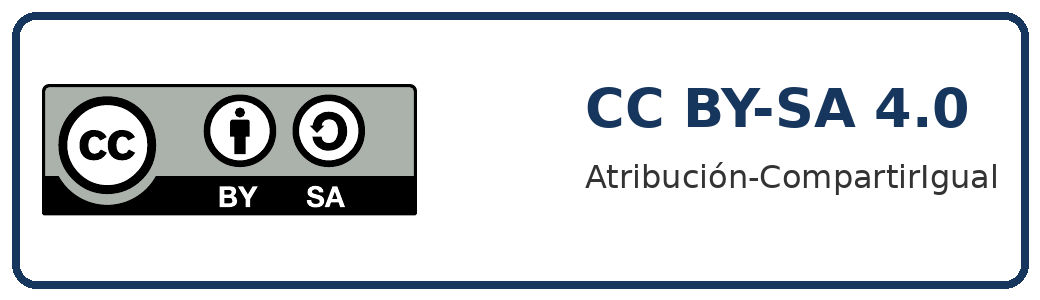
\includegraphics[height=0.52cm]{images/cc_by_sa_4_0.png}}
\newcommand{\openvisual}[1]{%
\begin{tikzpicture}
  \node[draw=colorblue, rounded corners=3pt, fill=colorblue!6,
        minimum height=2.2cm, text width=0.78\linewidth, align=center,
        inner sep=8pt] {\textbf{#1}\\[0.35em]\scriptsize Esquema conceptual original de la edición abierta};
\end{tikzpicture}}
\setbeamertemplate{footline}{%
  \leavevmode%
  \hbox{%
    \begin{beamercolorbox}[wd=.82\paperwidth,ht=2.7ex,dp=1.1ex,leftskip=1em]{author in head/foot}%
      \scriptsize Material docente en abierto URJC · CC BY-SA 4.0
    \end{beamercolorbox}%
    \begin{beamercolorbox}[wd=.18\paperwidth,ht=2.7ex,dp=1.1ex,center]{date in head/foot}%
      \scriptsize\insertframenumber/\inserttotalframenumber
    \end{beamercolorbox}%
  }%
}

\begin{document}

\begin{frame}
\titlepage
\end{frame}

\begin{frame}{Licencia y datos de publicación}
\small
\begin{center}
\ccbadge
\end{center}
\textbf{Material docente en abierto de la Universidad Rey Juan Carlos}\\
\textbf{Asignatura:} Big Data Processing II\\
\textbf{Titulación:} Máster Universitario en Análisis de Datos Deportivos\\
\textbf{Autores:} Alberto Fernández Isabel \\ Natalia Madrueño Sierro \\ Rubén Rodríguez Fernández\\
\textbf{Fecha:} 2026\\[0.4em]
© 2026 Equipo docente. Algunos derechos reservados. Esta obra se distribuye bajo la licencia
\href{https://creativecommons.org/licenses/by-sa/4.0/deed.es}{Creative Commons Atribución-CompartirIgual 4.0 Internacional}.\\[0.4em]
Los logotipos, marcas y referencias de terceros conservan su régimen jurídico propio y quedan excluidos de la licencia, salvo indicación expresa.\\
\textbf{Depósito institucional:} \url{https://burjcdigital.urjc.es}
\end{frame}


\begin{frame}\frametitle{Objetivos del Tema}
\begin{itemize}
    \item Comprender la transición del análisis retrospectivo (BI tradicional) a la toma de decisiones prescriptiva en tiempo real.
    \item Diseñar infraestructuras integradas combinando ingestión masiva (Kafka) y cómputo continuo (Spark).
    \item Desplegar sistemas de IA generativa y ecosistemas multiagente sobre flujos de datos deportivos.
    \item Implementar arquitecturas RAG multimodales para la comprensión espacio-temporal del juego.
    \item Automatizar la generación de informes y narrativas adaptadas a diferentes perfiles de stakeholders.
\end{itemize}
\end{frame}

\begin{frame}\frametitle{Índice}
\tableofcontents
\end{frame}

% =====================================================
\section{Introducción: El paradigma del análisis automatizado}
\sectionpagetitle{Introducción al paradigma automatizado}

\begin{frame}\frametitle{Del Business Intelligence a la IA Prescriptiva}
\begin{itemize}
    \item La ciencia de datos deportivos ya no puede depender exclusivamente de los informes post-partido.
    \item El valor del dato decae exponencialmente desde el momento en que ocurre la acción.
    \item \textbf{Objetivo moderno:} Proveer a los entrenadores y analistas de herramientas que sugieran ajustes tácticos durante el desarrollo de la competición.
    \item Se exige una transición arquitectónica hacia la analítica predictiva y automatizada.
\end{itemize}
\end{frame}

\begin{frame}\frametitle{El ecosistema analítico moderno}
La infraestructura actual requiere la convergencia de tres pilares:
\begin{itemize}
    \item \textbf{Ingestión continua:} Captura ininterrumpida de biometría, GPS y vídeo.
    \item \textbf{Motor determinista:} Cálculos estadísticos en ventanas temporales.
    \item \textbf{Capa cognitiva (IA):} Modelos de lenguaje que interpretan y traducen matemáticas en táctica.
\end{itemize}
Esta convergencia permite pasar de paneles de control estáticos a \textbf{"sistemas observacionales" inteligentes}.
\end{frame}

\begin{frame}\frametitle{Límites de los modelos aislados}
\begin{itemize}
    \item Un LLM tradicional es una "foto fija" probabilística basada en su entrenamiento.
    \item \textbf{El problema en el deporte:} Carece de contexto del estado actual del mundo; no sabe quién está fatigado ni cuál es el marcador en el minuto 75.
    \item \textbf{Solución:} Integrar al LLM como un motor de razonamiento (\textit{reasoning engine}) dentro de un pipeline de datos alimentado en vivo.
\end{itemize}
\end{frame}

\begin{frame}\frametitle{La transición hacia el tiempo real}
\begin{itemize}
    \item La automatización total abarca desde la captura del evento micro-táctico hasta la narrativa macroscópica.
    \item Requiere superar los límites epistemológicos de los enfoques batch.
    \item El contexto inmediato permite extraer valor competitivo en la ventana crítica de la toma de decisiones.
\end{itemize}
\end{frame}

\begin{frame}\frametitle{Flujo general: De la telemetría a la decisión}
\begin{enumerate}
    \item \textbf{Fuentes (Productores):} Tracking óptico, sensores de balones, wearables.
    \item \textbf{Middleware de Mensajería:} Enrutamiento masivo y ordenado.
    \item \textbf{Motor de Streaming:} Agregación e identificación de anomalías.
    \item \textbf{Agentes LLM / RAG:} Generación de diagnósticos e informes.
    \item \textbf{Destinos (Consumidores):} Aplicaciones de cuerpo técnico, retransmisiones (broadcasters).
\end{enumerate}
\end{frame}

% =====================================================
\section{Arquitecturas completas de ingestión y procesamiento}
\sectionpagetitle{Arquitecturas completas de ingestión}

\begin{frame}\frametitle{El reto arquitectónico}
\begin{itemize}
    \item Entornos de alta presión (estadios repletos) con conectividad variable.
    \item \textbf{Teorema CAP aplicado al deporte:}
    \begin{itemize}
        \item Consistencia (C), Disponibilidad (A), Tolerancia a Particiones (P).
    \end{itemize}
    \item En un partido en directo, la latencia es crítica.
    \item Generalmente, se prioriza la \textbf{Disponibilidad} y la \textbf{Tolerancia a fallos} de red (AP) sobre la consistencia matemática perfecta que llegaría tarde.
\end{itemize}
\end{frame}

\begin{frame}\frametitle{Ingestión orientada a eventos (Kafka)}
\begin{itemize}
    \item Apache Kafka actúa como el núcleo de mensajería (Pub/Sub).
    \item \textbf{Desacoplamiento:} Los sensores (visión, GPS) no saben quién consume los datos.
    \item \textbf{Ventaja:} Permite que múltiples sistemas (motores de cálculo de xG, sistemas de IA generativa para alertas tácticas y bases de datos históricas) consuman el mismo evento de forma independiente y concurrente.
\end{itemize}
\end{frame}

\begin{frame}\frametitle{Esquemas de eventos deportivos}
\begin{itemize}
    \item Los proveedores de datos (Opta, StatsBomb) o estándares de la FIFA (EPTS) envían flujos jerárquicos.
    \item \textbf{Granularidad:} Un simple "pase" incluye decenas de metadatos asociados.
    \item La comprensión de estos esquemas JSON es vital para el diseño de bases de datos vectoriales y algoritmos analíticos.
\end{itemize}
\end{frame}

\begin{frame}\frametitle{Estructura de un mensaje táctico (Ejemplo)}
\begin{center}
\small
\begin{tabular}{l l >{\raggedright\arraybackslash}p{7.6cm}}
\hline
\textbf{Campo (Opta/EPTS)} & \textbf{Tipo} & \textbf{Implicación Analítica} \\
\hline
event\_id & UUID & Deduplicación semántica (exactly-once). \\
type\_id & Entero & Filtrado en capa de ingesta (separar pases de tiros). \\
start\_x, start\_y & Flotante & Coordenadas que alimentan modelos espaciales. \\
timestamp & Time & Reloj del evento, crítico para latencias. \\
qualifiers & JSON & Contexto profundo (presión, pie débil) para enriquecer prompts de la IA. \\
\hline
\end{tabular}
\end{center}
\end{frame}

\begin{frame}\frametitle{Optimización del clúster Kafka}
\begin{itemize}
    \item \textbf{Paralelismo horizontal:} El número de particiones define el rendimiento máximo.
    \[
    \text{Particiones} = \frac{\text{Throughput total deseado}}{\text{Velocidad máxima del consumidor}}
    \]
    \item \textbf{Eficiencia:} Afinación de \texttt{batch.size} y \texttt{linger.ms} combinados con compresión (Snappy/Gzip) para reducir la carga de red.
    \item \textbf{Resiliencia:} Uso de \texttt{acks=all} y \texttt{enable.idempotence=true} para garantizar que ningún dato crítico (como una alerta de fatiga) se pierda o duplique.
\end{itemize}
\end{frame}

\begin{frame}\frametitle{Cómputo continuo con Spark Structured Streaming}
\begin{itemize}
    \item Se trata al flujo ininterrumpido de eventos como una tabla relacional en crecimiento perpetuo.
    \item Permite a los científicos de datos abstraerse de la complejidad subyacente.
    \item Motor de cálculo incremental para preparar métricas (ej. Posesión en el último tercio) antes de enviarlas al modelo de IA generativa.
\end{itemize}
\end{frame}

\begin{frame}\frametitle{Semántica Exactly-Once y Estado}
\begin{itemize}
    \item En un estadio, los dispositivos se desconectan y reconectan continuamente.
    \item Spark gestiona la semántica exactly-once usando:
    \begin{itemize}
        \item \textbf{Write-Ahead Logs (WAL)} en sistemas distribuidos persistentes (HDFS/S3).
        \item \textbf{Checkpointing distribuido:} Guarda el progreso de manera asíncrona.
    \end{itemize}
    \item Asegura que el LLM no reciba alertas duplicadas sobre el mismo evento de juego.
\end{itemize}
\end{frame}

\begin{frame}\frametitle{Event-Time y Watermarking}
\begin{itemize}
    \item \textbf{Problema de asincronía:} El retraso entre que el jugador hace el sprint y el paquete de datos llega al servidor en la nube.
    \item \textbf{Watermarking:} Umbral temporal de gracia que el sistema espera antes de cerrar el cálculo de una ventana.
    \[
    W(t) = T_{max}(t) - \Delta
    \]
    \item Garantiza que la IA analice ventanas de tiempo completas sin colapsar la memoria del servidor.
\end{itemize}
\end{frame}

\begin{frame}\frametitle{Predominio de la Arquitectura Kappa}
\begin{itemize}
    \item \textbf{Desventaja de Lambda:} Mantener código dual (Speed y Batch) duplica el riesgo de error algorítmico.
    \item \textbf{Ventaja de Kappa para la IA:} Kafka persiste todo el historial; el motor de streaming reprocesa todo desde cero si cambia un modelo subyacente.
    \item Garantiza que el agente cognitivo de IA reciba distribuciones de datos y métricas idénticas, ya sea auditando un partido de 2024 o analizando el directo.
\end{itemize}
\end{frame}

% =====================================================
\section{Orquestación de IA Generativa y flujos agénticos}
\sectionpagetitle{IA Generativa y flujos agénticos}

\begin{frame}\frametitle{De la interacción reactiva a la agéntica}
\begin{itemize}
    \item La interacción ya no es reactiva (humano preguntando a una máquina).
    \item Se avanza hacia arquitecturas \textbf{agénticas y orquestadas orientadas a la acción} (Agentic Workflows).
    \item Un agente no solo resume texto, sino que ejecuta código, consulta bases de datos vectoriales y planifica respuestas estructuradas.
\end{itemize}
\end{frame}

\begin{frame}\frametitle{Capa de abstracción con LangChain}
\begin{itemize}
    \item LangChain funciona como el marco orquestador.
    \item Interconecta el razonamiento del LLM con las capacidades deterministas de Big Data (Spark, bases de datos SQL).
    \item Aporta "herramientas" (Tools) al LLM para que este no invente números, sino que los busque activamente en los clústeres de datos.
\end{itemize}
\end{frame}

\begin{frame}\frametitle{Integración Text-to-SQL en Spark}
\textbf{Uso práctico:} Un analista interroga al sistema en lenguaje natural.
\begin{enumerate}
    \item El LLM usa su herramienta integrada para traducir la consulta humana a un código de consulta (Spark SQL).
    \item Ejecuta la consulta contra el DataFrame en memoria.
    \item Extrae el resultado numérico.
    \item Redacta una explicación en base a ese dato duro.
\end{enumerate}
\end{frame}

\begin{frame}\frametitle{Flujo Planner-Executor en análisis táctico}
\textbf{Pregunta del entrenador:} "¿Tasa de éxito de pase progresivo del mediocentro bajo presión en los últimos 15 min?"
\begin{itemize}
    \item \textbf{Planner:} Descompone la consulta $\rightarrow$ Entidad (jugador), Métrica (tasa de pase), Contexto (presión alta basada en coordenadas), Filtro Temporal (15 min).
    \item \textbf{Executor:} Corre el SQL en Spark.
    \item \textbf{Synthesizer:} Valida lógicamente el 45\% obtenido y genera la alerta narrativa argumentada.
\end{itemize}
\end{frame}

\begin{frame}\frametitle{Hacia los Agentic Workflows}
\begin{itemize}
    \item La automatización proactiva que monitorea patrones complejos sin requerir un prompt humano.
    \item Se utilizan máquinas de estado explícitas para enrutar decisiones.
    \item Compañías como \textbf{Machina Sports} ya proveen infraestructuras de IA agéntica enfocadas exclusivamente en el ecosistema deportivo, dotando a la IA de conocimiento táctico profundo y ejecución fiable.
\end{itemize}
\end{frame}

\begin{frame}\frametitle{Patrón ReAct (Reasoning + Acting) en tiempo real}
El sistema opera en un ciclo de iteración continuo:
\begin{enumerate}
    \item \textbf{Think:} "Detecto una anomalía en la velocidad del jugador."
    \item \textbf{Act:} "Usaré la herramienta de historial médico para ver sus promedios."
    \item \textbf{Observe:} "La recuperación cardíaca ha bajado un 15\% respecto al mes pasado."
    \item \textbf{Act:} "Emitiré una alerta de sustitución al cuerpo técnico."
\end{enumerate}
\end{frame}

\begin{frame}\frametitle{Control de flujo en agentes autónomos}
Para garantizar estabilidad computacional frente a alucinaciones:
\begin{itemize}
    \item \textbf{Router:} Desvía consultas puramente estadísticas hacia motores deterministas y consultas cualitativas hacia RAG.
    \item \textbf{Validator:} Obliga al agente a parsear su salida bajo un formato estricto (JSON), repitiendo el proceso si el formato es erróneo.
    \item \textbf{Loop Bounded:} Impone un máximo de "pensamientos" iterativos para evitar que el sistema agote los tokens en un bucle infinito de resolución.
\end{itemize}
\end{frame}

% =====================================================
\section{RAG Multimodal y Generación de Narrativas}
\frame{\sectionpage}

\begin{frame}\frametitle{Más allá de los datos tabulares}
\begin{itemize}
    \item Los datos tabulares solo representan una fracción de la realidad del partido.
    \item \textbf{RAG Multimodal:} Integrar simbióticamente flujos de vídeo HD, audio de retransmisión y telemetría estructurada.
    \item \textbf{Vectorización combinada:} Permite a la IA no solo buscar "tiros a puerta", sino buscar "jugadas con presión asfixiante" utilizando comprensión espaciotemporal.
\end{itemize}
\end{frame}

\begin{frame}\frametitle{Alineación Visual y Textual}
\begin{itemize}
    \item Sistemas de visión profunda analizan fotogramas y detectan la topología del juego y trayectorias.
    \item \textbf{Arquitecturas avanzadas (ej. GameSight):} Realizan un alineamiento en dos etapas, identificando primero las entidades visuales anónimas en el vídeo para luego enriquecerlas con metadatos y estadísticas históricas.
    \item Esto mejora drásticamente la calidad de los comentarios automatizados.
    \item Erradica la disonancia de contexto en los modelos de lenguaje genéricos.
\end{itemize}
\end{frame}

\begin{frame}\frametitle{El desafío Data-to-Text}
\begin{itemize}
    \item \textbf{Problema fundamental:} Inyectar payloads JSON crudos al contexto del LLM es ineficiente y provoca pérdida de precisión matemática (alucinaciones).
    \item \textbf{Solución:} Preprocesamiento determinista.
    \item Traducir diccionarios numéricos (\texttt{type\_id = 10}, \texttt{outcome = 0}) a oraciones semánticas estructuradas antes del prompt: "El jugador X intentó una entrada pero no recuperó la posesión".
\end{itemize}
Cada ve es menos necesaria esta conversión, pero no es deseable introducir JSONs muy grandes.
\end{frame}

\begin{frame}\frametitle{Redacciones Autónomas (Autonomous Newsrooms)}
\begin{itemize}
    \item Creación de pipelines cerrados de monitorización continua de eventos para generar contenido automatizado y filtrado.
    \item Sistemas como \textbf{LLM-SportTweet} utilizan orquestación para leer flujos de eventos asíncronos y tomar decisiones editoriales determinando qué sucesos merecen ser convertidos en narrativas.
\end{itemize}
\end{frame}

\begin{frame}\frametitle{Scoring Multidimensional en eventos}
Antes de generar una alerta o informe, el LLM evalúa y puntúa internamente el evento táctico o la noticia:
\begin{itemize}
    \item \textbf{Proximity:} Relevancia para el deporte/equipo analizado.
    \item \textbf{Freshness:} Criticidad e inmediatez del suceso.
    \item \textbf{Impact:} Grado de influencia en el resultado del partido.
    \item \textbf{Uniqueness:} Penalización de la redundancia frente a la memoria episódica a corto plazo.
\end{itemize}
\end{frame}

\begin{frame}\frametitle{Síntesis condicionada (Prompting estructurado)}
\begin{itemize}
    \item Solo si el evento supera el umbral de Scoring, el agente desencadena la generación.
    \item \textbf{Técnicas Few-Shot:} Forzar al modelo a adoptar un formato retórico y una longitud específica.
    \item Se adapta el vocabulario automáticamente:
    \begin{itemize}
        \item \textbf{Modo Analista:} Foco estadístico en métricas de presión.
        \item \textbf{Modo Aficionado:} Foco emocional y contexto histórico para redes sociales.
    \end{itemize}
\end{itemize}
\end{frame}

\begin{frame}\frametitle{Modelos híbridos para baja latencia}
\begin{itemize}
    \item La generación de narrativas en directo exige reducir la latencia al mínimo.
    \item Se investigan soluciones híbridas que acoplan redes neuronales convolucionales con LLMs.
    \item \textbf{Ejemplo:} Arquitecturas OS-CNN pre-computan y anticipan eventos cinemáticos que luego se inyectan en plantillas Prompt Engineering para modelos como LLaMA 3.3, logrando comentarios fluidos en tiempo real con latencias aptas para retransmisiones interactivas.
\end{itemize}
\end{frame}

\begin{frame}\frametitle{Mitigación sistémica de alucinaciones}
La fiabilidad estricta no es opcional en la élite.

\vspace{0.3em}
\textbf{Principio de Separación (Separation of Concerns):}
\begin{itemize}
    \item El LLM jamás computa matemáticas (complejas).
    \item El motor Spark realiza las agregaciones.
    \item El marco RAG localiza el dato duro.
    \item El LLM ingiere el dato protegido bajo el mandato estricto de "Utilice EXCLUSIVAMENTE los parámetros de la matriz".
\end{itemize}
\end{frame}

% =====================================================
\section{Visualización avanzada e interfaces conversacionales}
\sectionpagetitle{Visualización Avanzada e Interfaces}

\begin{frame}\frametitle{Democratización de los insights}
\begin{itemize}
    \item Los petabytes de datos son inútiles sin una democratización efectiva de los insights.
    \item \textbf{El paradigma 2026:} Las predicciones y gráficas estáticas previas al partido son obsoletas.
    \item Se demandan probabilidades recalibradas continuamente en función del flujo de eventos (e.g., probabilidades de micro-sucesos) y total transparencia analítica.
\end{itemize}
\end{frame}

\begin{frame}\frametitle{Personalización a escala (Stakeholders)}
\begin{itemize}
    \item \textbf{Cuerpo Técnico:} Resolución analítica máxima; fusión de cinemática de alta frecuencia y fisiología para prevención biomecánica de lesiones.
    \item \textbf{Front Office:} Proyecciones a largo plazo (impacto económico, modelado de carreras de atletas).
    \item \textbf{Broadcasters:} Baja latencia, inmersión rápida. Respuestas dinámicas a escenarios de tipo "What-If" para los espectadores.
\end{itemize}
\end{frame}

\begin{frame}\frametitle{Interfaces conversacionales}
\begin{itemize}
    \item Sustitución de los paneles pasivos (Tableau, Power BI clásicos) por ecosistemas interactivos.
    \item La IA funciona como "científico de datos virtual permanente".
    \item Permite a los analistas realizar consultas declarativas profundas (e.g., "Compara nuestro índice de progresión central antes y después de la sustitución del minuto 60").
\end{itemize}
\end{frame}

\begin{frame}\frametitle{Explicabilidad inmersiva del dato}
\begin{itemize}
    \item \textbf{Problema de los Black-Boxes:} Los cuerpos técnicos no confían en índices predictivos opacos.
    \item La visualización debe incluir \textbf{Virtual Analyst Narratives}.
    \item El sistema no solo emite una probabilidad del 73\%, sino que el agente detalla causalidades (e.g., métricas previas, tendencias posicionales) para justificar el número mostrado en pantalla.
\end{itemize}
\end{frame}

\begin{frame}\frametitle{Chain-of-Thought aplicado a visualización}
\begin{enumerate}
    \item \textbf{Recepción:} El agente capta el pico en la gráfica.
    \item \textbf{Consulta interna:} Formula SQL y consulta el stream de datos en segundo plano.
    \item \textbf{Recuperación RAG:} Acopla métricas actuales con cortes de vídeo del partido en curso.
    \item \textbf{Generación de la narrativa:} Ofrece una síntesis causal explicativa en lenguaje natural para acompañar al gráfico.
\end{enumerate}
\end{frame}

\begin{frame}\frametitle{Gestión paramétrica de la Latencia}
\begin{itemize}
    \item \textbf{Time-to-Insight:} Métrica fundacional en el desarrollo de paneles intra-partido.
    \item \textbf{Problema:} La decodificación del modelo generativo añade un retraso inherente.
    \item \textbf{Solución (Streaming UI):} Reducir el Time To First Token (TTFT) inyectando la respuesta palabra por palabra a la interfaz (vía WebSockets).
    \item Se mitiga la percepción de lentitud del usuario final de forma drástica.
\end{itemize}
\end{frame}

\begin{frame}\frametitle{Priorizar la Disponibilidad en vivo}
\begin{itemize}
    \item Durante la competición táctica, la fluidez del panel de control es primordial.
    \item Frente al teorema CAP, el diseño del panel favorece la tolerancia a la partición y la disponibilidad.
    \item Es preferible renderizar tendencias estimadas al instante que bloquear el dashboard a la espera de la consistencia total del evento cerrado.
\end{itemize}
\end{frame}

% =====================================================
\section{Conclusiones}
\frame{\sectionpage}

\begin{frame}\frametitle{Conclusiones}
\begin{itemize}
    \item El procesamiento de Big Data moderno consolida el streaming continuo con el análisis cognitivo.
    \item La orquestación agéntica y los RAG multimodales son las claves para dar contexto espacio-temporal a la inteligencia artificial.
    \item La arquitectura debe mitigar sistemáticamente las alucinaciones limitando el acceso de los modelos a datos precomputados deterministas.
    \item El futuro radica en visualizaciones conversacionales y proactivas que empoderen a todos los stakeholders del entorno deportivo en tiempo real.
\end{itemize}
\end{frame}



\begin{frame}{Fuentes, imágenes y reutilización}
\small
\begin{itemize}
  \item El texto, los ejemplos y los esquemas de esta edición abierta se distribuyen bajo CC BY-SA 4.0.
  \item Las imágenes de procedencia no acreditada de la versión de trabajo se han retirado y sustituido por esquemas conceptuales originales.
  \item Los logotipos y marcas citados se utilizan únicamente con finalidad identificativa y quedan excluidos de la licencia.
  \item Las referencias técnicas se conservan mediante citas y enlaces a sus fuentes correspondientes.
  \item Información de licencia: \url{https://creativecommons.org/licenses/by-sa/4.0/deed.es}
\end{itemize}
\end{frame}

\end{document}
